%
%  発表会の原稿
%
%\documentstyle[fancyheadings,11pt,twocolumn,rise]{jarticle}
\documentclass[11pt,twocolumn]{jarticle}
\usepackage{fancyheadings}
\usepackage{rise}
\usepackage[dvipdfmx]{graphicx}
%
\begin{document}
%\small
\title{\Large 調査項目の拡張しやすさを考慮した\\ソースコード解析システムの構築}
\author{19T305 \ 小方~亮人 (香川研究室)}
%
\abstract{
プログラミングを学び始めたばかりの初学者は
コンパイル時のエラー内容を理解することが困難である。
本研究では入力されたソースコードに対して解析を行い、
間違っている箇所を指摘するシステムを構築した。解析には
Haskellを用い、調査項目の拡張性が期待できる。
}
\maketitle
\pagestyle{headings}
\thispagestyle{headings}
%
\section{はじめに}
学習者がC言語を学び始めたばかりの時、
コンパイルした際に表示されるエラーや警告が
何を意味しているのかが分からず、
エラーの修正に多くの時間をかけてしまうことが多々ある。
初学者によくある間違いに対して
より明確なエラーメッセージを出力することで、
エラーの修正が的確に行えるようになり
学習効率が向上すると考えられる。
また、プログラミング学習者がソースコードを記述する際に
犯す間違いには様々な種類がある。
エラーを指摘するシステムを構築した時点で
その全ての間違いを網羅することは
不可能であり、システムを運用していくにつれて
エラーの調査項目を増やす必要がある。
そのため、エラー指摘システムには
新しく調査したい調査項目が
できた時に容易にシステムに組み込むことが
できる拡張性が求められる。

\section{先行研究}
島川の研究 \cite{1}はC言語を初めて学ぶ学習者によくある
間違いに対して理解の容易なエラーメッセージを表示しエラーの修正を補助する機能を持つ。
これにより簡易な質問数が減少することで学習効率の向上や指導者の負担軽減を図っている。
しかしこのシステムで利用しているC-Helper \cite{2}が実装に用いているJavaでは
構文解析結果である構文木を扱う際にVisitorパターンというデザインパターンが
用いられている。新しく調査項目を増やそうとする場合、新しいメソッドの追加と
各クラスにそのメソッドに応じた実装を追加する必要があるため、
調査できる項目の拡張性に優れていない。
この問題点に対してHaskellを用いて解決を試みた研究が木村の研究 \cite{3}である。
木村の研究はソースコードのエラー箇所をハイライトすることで
教育者の添削を支援するものである。しかし学習者に対して即座に
ミスのフィードバックを示すことはできず、教育者に対しても
エラー指摘の完全な自動化は図られていない。
そこで本研究では、実装にHaskellを用いることで容易に調査項目を増やすことができ、
学習者に即座にフィードバックを行うことができるシステムを構築することを目的とする。

\section{システムの実装}
本研究ではHaskellとそのライブラリであるlanguage-c-quoteを用いてシステムの実装を行う。
Haskellには参照透過性や静的型付けといった関数型言語に
多く採用されている機能に加え、パターンマッチや型推論、モナドなどの特徴的な機能がある。
これらの機能を組み合わせることで構文木のようなデータ型を扱う際に
命令型言語に比べてHaskellはより簡潔かつ容易に関数を実装できることが期待される。
language-c-quoteはC言語の構文解析を行うHaskellのライブラリであり、
解析結果が扱いやすいため、新しく調査項目を増やす際に容易に
プログラムに追加することができると考えた。
また、Webベースで実装を行うことでシステムのインストールを不要とし、
利用者側と開発側が双方ともにシステム導入に関する負担が軽減されることを目指した。

本研究のシステムは、ブラウザ上のテキストエリアの入力フォームに
入力されたソースコードを文字列として受け取り
language-c-quoteによって構文解析を行う。その結果から
初学者が間違いを起こしやすいif文などの情報を
抜き出し、間違った記述をしていないか調査を行う。
本システムで調査できる項目は、インデントのミス、printfやscanfの
受け取る変数の数が間違っているミス、if文の条件式が
関係演算子による式ではなく代入式になっているミス、
関数名が他の関数と重複しているミス、
返却値がint型の関数にreturnが記述されていないミスがある。
間違っている箇所の行番号とその内容を
HTMLファイルに書き込み、解析結果を
表示するページに出力する。この出力表示では入力されたソースコードと
ソースコードの間違っている行番号の色を変更して表示しているため、
視覚的にエラー箇所を理解することができる。
以下にソースコードの入力画面 (図\ref{fig:sys1}) と
解析結果の表示画面 (図\ref{fig:sys2})を示す。

\begin{figure}[!h]
   \begin{center}
      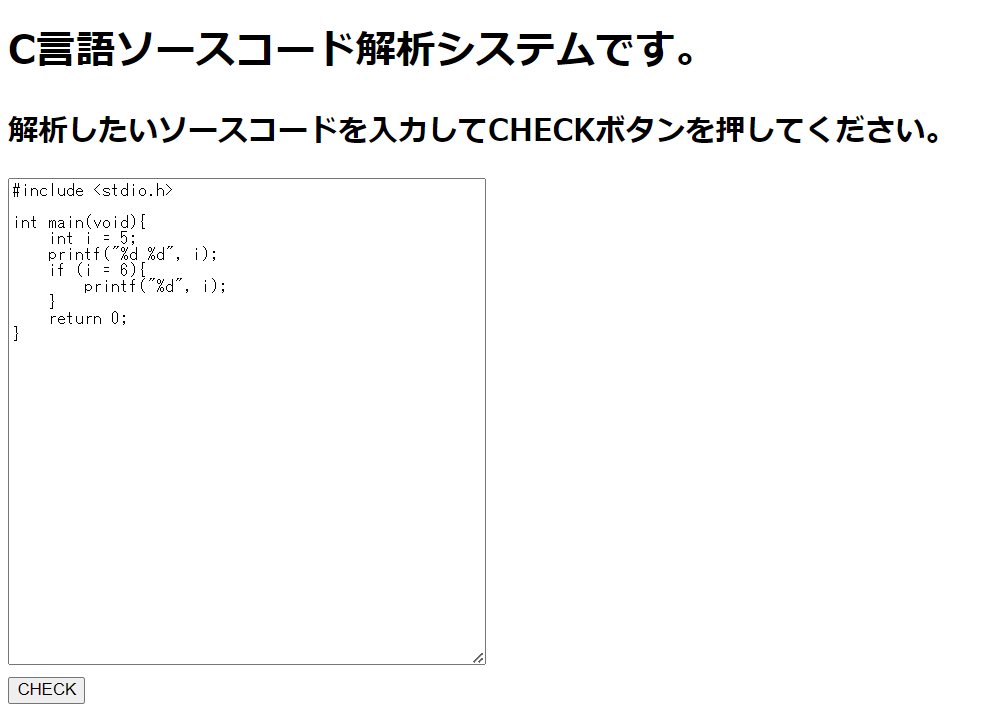
\includegraphics[width=8cm]{systempage1.png}
      \caption{ソースコード入力画面}
      \label{fig:sys1}
   \end{center}
\end{figure}

\begin{figure}[!h]
   \begin{center}
      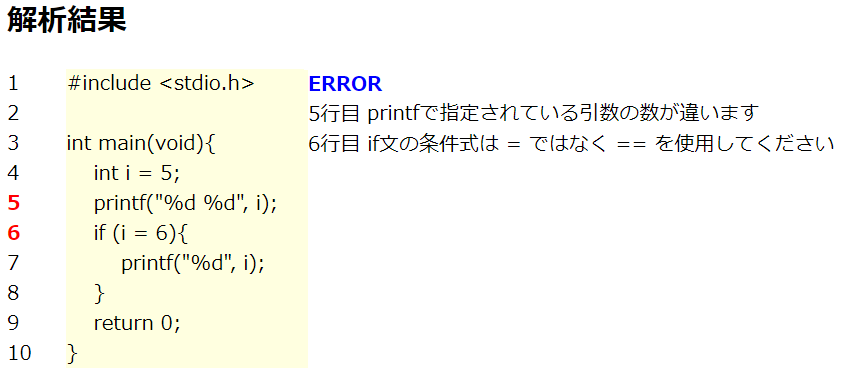
\includegraphics[width=8cm]{systempage2.png}
      \caption{解析結果表示画面}
      \label{fig:sys2}
   \end{center}
\end{figure}

\section{まとめ}
本研究では、プログラミング初学者向けのソースコード解析システムの
構築を行った。インデントのミス等の初学者が犯しがちな
ミスに対して調査を行う機能をWebベースシステムで実装することに成功した。
また、ソースコード構文解析結果からHaskellによって調査したい構文の
箇所を抜き出して調査を行っているため、Haskellの知識さえあれば
調査項目を容易に拡張することが可能である。

しかし、現状で調査することが可能な項目の数は
少なく早急な調査項目の追加が求められる。
またHaskellの知識が必要なことから、調査項目の拡張についての
評価実験を行うことが困難であったため拡張しやすさに関する
評価は筆者の主観的なものでしかない。そのため
実際にHaskellを学ぶ講義で追加する調査項目のコードを記述する課題を
出したり、知識がなくても調査のイメージをつかめるように
分かりやすさを重視したビジュアルプログラミングを利用したり
といった方法で解決を図る必要がある。


%----------------------------------
\begin{thebibliography}{9}
%
\bibitem{1}
島川 大輝, 香川 考司, ``C-Helperを用いたWebベースのC言語開発環境の構築'',

教育システム情報学会第40回全国大会 (JSiSE2015) 講演論文集, A3-1, 2015.

\bibitem{2}
サイボウズ・ラボユース Ucida Kota, \\ ``C-Helper GitHub'',

https://github.com/uchan-nos/c-helper \\ (閲覧日:2023年2月)

\bibitem{3}
木村 光星, 香川 考司, ``構文解析を用いた\\C言語指導コメント支援システムの構築'',

教育システム情報学会 (JSiSE) 2018年度 \\ 第4回研究会, 2018

\end{thebibliography}
\end{document}
